% vim: set textwidth=78 autoindent:

\subsection{Plugins Decorativi}

% when the revision of a section has been finalized, 
% comment out the following line:
% \updatedisclaimer

I plugin decorativi includono il plugin Etichetta diritti d'autore, il plugin Freccia nord ed il plugin Barra di scala. Sono usati per "decorare" la mappa aggiungendo elementi cartografici.

\subsubsection{Plugin Etichetta diritti d'autore}

Il nome del plugin è un po' fuorviante, in realtà si può aggiungere qualsiasi testo alla mappa.

\begin{figure}[ht]
   \begin{center}
   \caption{Plugin Etichetta di Copyright \nixcaption}\label{fig:copyright}\smallskip
   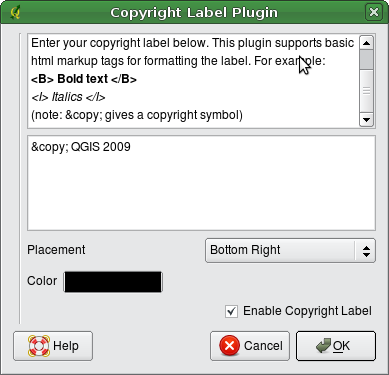
\includegraphics[clip=true, width=8cm]{copyright}
\end{center}  
\end{figure}

\begin{enumerate}
\item Assicurarsi che il plugin sia caricato
\item Selezionare su \mainmenuopt{Plugins} > \dropmenuopt{Decorazioni} > \dropmenuopttwo{copyright_label}{Etichetta di Copyright} o selezionare il pulsante \toolbtntwo{copyright_label}{Etichetta di Copyright} dalla barra degli Strumenti.
\item Digitare il testo che si vuole aggiungere alla mappa. Si può usare il codice HTML come mostrato nell'esempio
\item Scegliere il posizionamento dell'etichetta dal menu a tendina \selectstring{Posizione}{In basso a destra}
\item Assicurasi che la casella \checkbox{Abilita etichetta di Copyright} sia selezionata
\item Premere \button{OK} 
\end{enumerate}

Nell'esempio sopra, la prima linea è in grassetto, la seconda (creata usando 
\textless br\textgreater) contiene un simbolo di copyright, seguito dal nome della nostra compagnia in corsivo.

\subsubsection{Plugin Freccia nord}

Il plugin Freccia nord aggiunge alla mappa una semplice freccia indicante il nord. Al momento c'è un solo stile disponibile. Si può aggiustare manualmente l'angolo della freccia o lasciare che QGIS indichi automaticamente la direzione. Se si sceglie di lasciar fare a QGIS, il programma fa la sua migliore congettura circa come la freccia dovrebbe essere orientata. Per il posizionamento della freccia si hanno quattro possibilità, corrispondenti ai quattro angoli della mappa.

\begin{figure}[ht]
   \begin{center}
   \caption{Plugin Freccia nord \nixcaption}\label{fig:north_arrow}\smallskip
   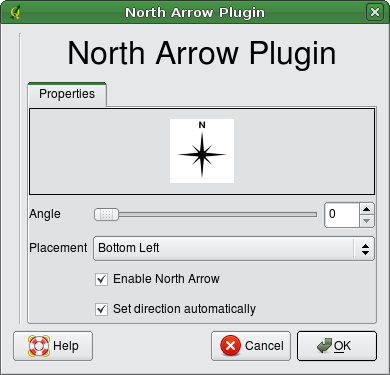
\includegraphics[clip=true, width=8cm]{north_arrow_dialog}
\end{center}  
\end{figure}

\subsubsection{Plugin Barra di Scala }
Il plugin Barra di scala aggiunge una semplice barra di scala alla mappa. Si può controllare lo stile ed il posizionamento, come anche l'etichettatura della scala.

QGIS supporta solamente di mostrare la scala nella stessa unità di misura della mappa. Cioè, se l'unità di misura dei layer è il metro, non si può creare una mappa in piedi. Allo stesso modo, se si usano gradi decimali, non si può creare una barra di scala che mostri le distanze in metri.

Per aggiungere una barra di scala:

\begin{enumerate}
\item Selezionare \mainmenuopt{Plugins} > \dropmenuopt{Decorazioni} > \dropmenuopttwo{scale_bar}{Barra di Scala} o premere il pulsante \toolbtntwo{scale_bar}{Barra di Scala} dalla barra degli Strumenti.
\item Scegliere il posizionamento dal menu a tendina \selectstring{Posizionamento}{In basso a sinistra}
\item Scegliere lo stile dalla lista \selectstring{Stile della Barra di Scala}{Porta in basso}
\item Scegliere il colore della barra di scala \selectcolor{Colore della barra}{black} o usare il colore nero di default
\item Impostare la dimensione della barra e la sua etichetta \selectnumber{Dimensione della barra}{30 gradi}
\item Assicurarsi che la casella \checkbox{Abilita barra di scala} sia selezionata
\item Se si vuole, scegliere di arrotondare automaticamente il numero quando la mappa viene ridimensionata \checkbox{Arrotonda automaticamente il numero durante il ridimensionamento}
\item Premere \button{OK} 
\end{enumerate} 

\begin{figure}[ht]
   \begin{center}
   \caption{Plugin Barra di Scala \nixcaption}\label{fig:scale_bar}\smallskip
   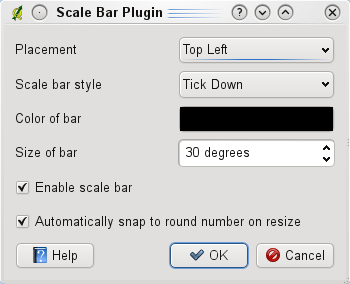
\includegraphics[clip=true, width=8cm]{scale_bar_dialog}
\end{center}  
\end{figure}
